\section*{7. \"Ubung (Abgabe: 16.06.2010, 8.30 Uhr, schriftlich)}

\subsection*{1.a. Wie stark muss man ein n-dimensionales Signal gl\"atten, um die Standardabweichung des Rauschens zu halbieren?}

\begin{align*}
Gegeben:\; \sigma_{reduced\;noise}^{2} &\approx \frac{1}{(2\sqrt{\pi}\sigma_{Gauss})^{n}} \sigma_{noise}^{2} \\
Ansatz:\; \sigma_{reduced\; noise} &:= \frac{1}{2}\sigma_{noise} \\
(\frac{1}{2}\sigma_{noise})^{2} &\approx \frac{1}{(2\sqrt{\pi}\sigma_{Gauss})^{n}} \sigma_{noise}^{2} \\
\frac{1}{2}\sigma_{noise} &\approx \frac{1}{(2\sqrt{\pi}\sigma_{Gauss})^{\frac{n}{2}}} \sigma_{noise},\; \sigma_{noise}>0 \\
\frac{1}{2} &\approx \frac{1}{(2\sqrt{\pi}\sigma_{Gauss})^{\frac{n}{2}}} \\
2 &\approx (2\sqrt{\pi}\sigma_{Gauss})^{\frac{n}{2}} \\
4 &\approx (2\sqrt{\pi}\sigma_{Gauss})^{n} \\
\sqrt[n]{4} &\approx 2\sqrt{\pi}\sigma_{Gauss} \\
\sqrt[n]{4}\cdot\frac{1}{2\sqrt{\pi}} &\approx \sigma_{Gauss} \\
\end{align*}
Das bedeutet, je mehr Dimensionen das Eingangssignal hat, desto geringer muss die Gl\"attung ausfallen, um die Standardabweichung des Rauschens zu halbieren.

\begin{figure}[!h] %  figure placement: here, top, bottom, or page
   \centering
   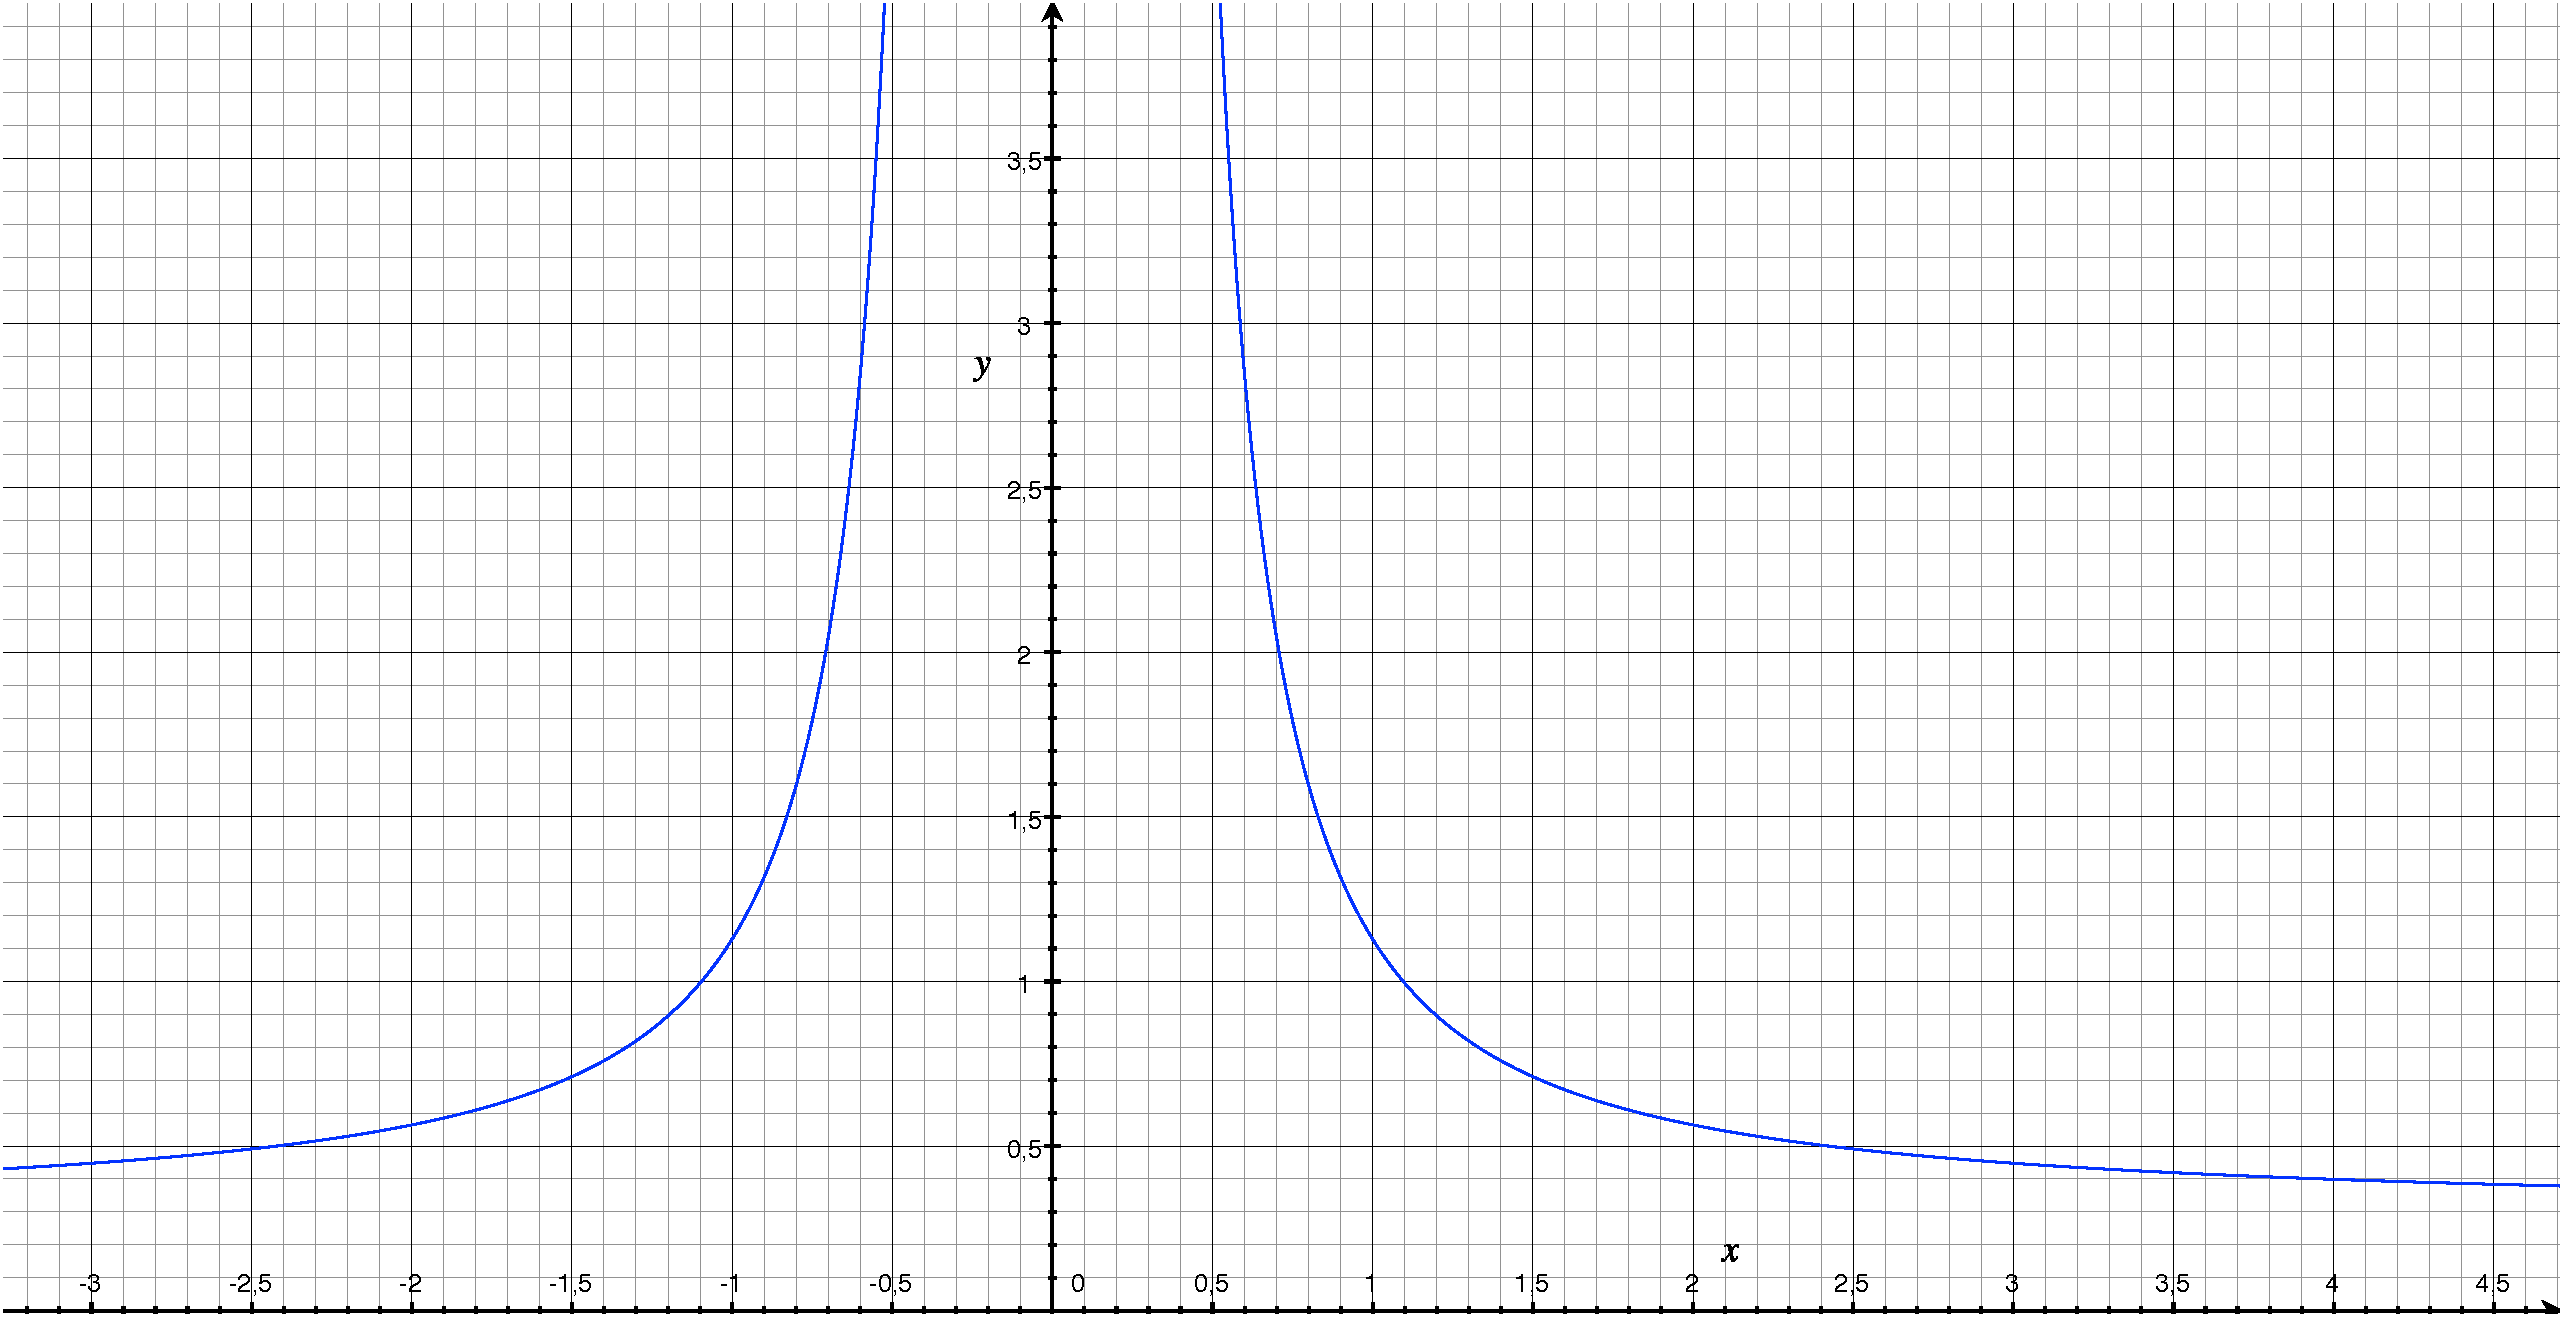
\includegraphics[height=0.17\textheight]{Uebung7/1_a.pdf} 
   \caption{Zusammenhang von Dimension (x$=\mid n \mid$) und Gl\"attung (y$=\sigma_{Gauss}$)}
   \label{fig:5.1}
\end{figure}

\subsection*{1.b. Auf welche Weise h\"angt die Varianz des Lokalisierungsfehlers f\"ur die F\"alle n=1,2,3 von dem Grad des urspr\"unglichen Rauschens und dem Grad der Gl\"attung ab? Was bedeutet das f\"ur die Anwendung von schwellenwertbasierten Kantendetektoren in verrauschten zweidimensionalen Bildern?}

Gesucht: \; Verh\"altnis $\mu$ zu $\sigma_{noise}$ und $\sigma_{Gauss}$ \\
\begin{align*}
\mu = Erwartungswert, \;
\sigma &= Standardabweichung, \;
\sigma^{2} =Varianz \\
f(x) &=\begin{cases}
\begin{array}{c}
\frac{1}{2} \\
-\frac{1}{2}
\end{array} & \begin{array}{c}
x>0\\
x\leq0
\end{array}\end{cases} \\
g(x) &= \frac{1}{\sigma_{Gauss}\sqrt{2\pi}}e^{-\frac{1}{2}(\frac{x-\mu}{\sigma_{Gauss}})^{2}}, \; \int_{A}\rightarrow1 \\
\mu &= \frac{\frac{1}{(2\sqrt{\pi}\sigma_{Gauss})^{n}}\sigma_{noise}^{2}}{(f_{b}^{'}(0))^{2}} \\
f_{b}(x) &= f(x)*g(x) \\
&= F^{-1}(F(x)\cdot G(x)) \\
F(x) &= \int_{-\infty}^{\infty}\frac{1}{\sigma_{Gauss}\sqrt{2\pi}}e^{-\frac{1}{2}(\frac{x-\mu}{\sigma_{Gauss}})^{2}}
\cdot e^{-j\omega x}dx
\cdot (\int_{-\infty}^{0}-\frac{1}{2}e^{-j\omega x}dx+\int_{0}^{\infty}\frac{1}{2}e^{-j\omega x}dx)
\end{align*}
Integral der normierten Gauss-Funktion ist 1. Leider ergibt sich aus der Substraktion der weiteren Integrale 0 und l\"asst so keine weiteren Interpretationen zu!?
